Para el capacitor de salida se utilizó un capacitor electrolítico de 
\(10\,\mu\text{F}\). En la hoja de datos se observa que la capacitancia real 
no se mantiene constante con la frecuencia, sino que está especificada respecto 
de \(C_0\), medida a \(20^\circ\text{C}\) y \(100\,\text{Hz}\) (ver \cite{Vishay_030031AS}.). Como se ve en la 
Figura~\ref{fig:cap_vs_freq}, a frecuencias altas la capacitancia efectiva disminuye 
de forma apreciable.

\begin{figure}[H]
    \centering
    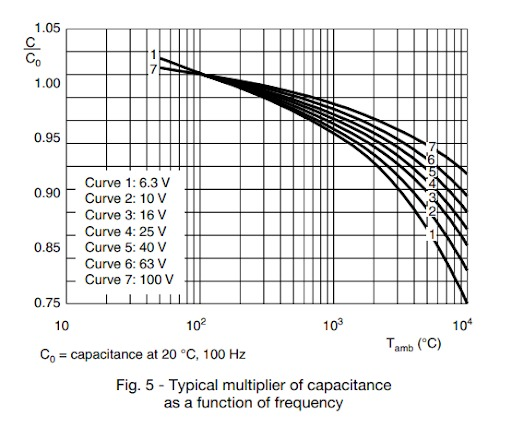
\includegraphics[width=0.65\textwidth]{img/PCB/capacitancia-vs-frecuencia.jpeg}
    \caption{Variación típica de la capacitancia efectiva normalizada respecto 
    de \(C_0\) en función de la frecuencia.}
    \label{fig:cap_vs_freq}
\end{figure}

Esto es importante porque la \textit{buck} opera con una frecuencia de conmutación del 
orden de $f_s \simeq 130\,\text{kHz}$.


Por lo tanto, el capacitor real no se comporta igual que el capacitor ideal de 
\(10\,\mu\text{F}\) usado en la simulación. En el modelo ideal, la corriente 
triangular del inductor es integrada por el capacitor.

\[
i_C(t)=C\frac{dv_o(t)}{dt}
\]

Por lo que el \textit{ripple} de tensión resulta más suavizado. En el circuito real se 
agregó además un capacitor cerámico de \(100\,\text{nF}\) en paralelo, con el 
objetivo de reducir la impedancia equivalente a altas frecuencias. Este capacitor 
ayuda a filtrar componentes rápidas y picos de conmutación, pero no reemplaza la 
función del capacitor electrolítico como elemento principal de almacenamiento de 
energía.

De esta forma, la diferencia entre la simulación y la medición puede explicarse 
porque el capacitor de salida no presenta una capacitancia efectiva constante a la 
frecuencia de trabajo. Como consecuencia, el ripple de salida puede verse menos 
integrado que en el modelo ideal, tomando una forma más triangular o tipo diente 
de sierra.